\documentclass{standalone}
\usepackage{tikz}
\usetikzlibrary{trees,automata, positioning, arrows}
\begin{document}
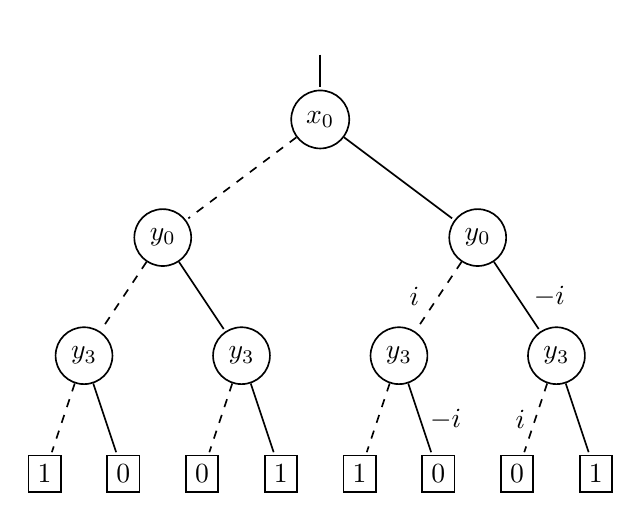
\begin{tikzpicture}[level 1/.style={sibling distance=4cm},
                    level 2/.style={sibling distance=2cm},
                    level 3/.style={sibling distance=1 cm, every node/.style={shape=rectangle,draw}},
                    level 4/.style={sibling distance=0.2 cm},
                    every node/.style={shape=circle, draw, align=center,solid},
                    edge from parent/.style={draw, solid, thick},
                    Lf/.style={edge from parent/.style={draw, dashed}},
                    Ri/.style={edge from parent/.style={draw, solid}},
                    semithick,auto,node distance=1cm,shorten >=1pt]
    \node (tree) {$x_0$}
    child [Lf] { % Dashed edge for Root to Lf
        node {$y_{0}$}
            child [Lf]{
            node {$y_3$} 
            child[Lf] 
                {node[solid] {$1$}} 
            child[Ri] 
                {node[solid] {$0$}}
            }
            child [Ri]{
            node {$y_3$} 
            child[Lf] 
                {node {$0$}} 
            child[Ri] 
                {node {$1$}}
            }
    }
    child [Ri] { % Dashed edge for Root to Lf
        node {$y_{0}$}
            child [Lf]{
            node {$y_3$} 
            child[Lf] 
                {node[solid] {$1$}} 
            child[Ri] 
                {node[solid] {$0$} edge from parent node[midway, right, draw = none] {$-i$}}
            edge from parent node[midway, left, draw = none] {$i$}}
            child [Ri]{
            node {$y_3$} 
            child[Lf] 
                {node {$0$} edge from parent node[midway, left, draw = none] {$i$}} 
            child[Ri] 
                {node[solid] {$1$}}
            edge from parent node[midway, right, draw = none] {$-i$}}
    };
    \node[state,draw=none,minimum size =0.001cm] (N) [above of=tree] {};
    \draw (N) -- (tree);
\end{tikzpicture}
\end{document}
